\documentclass[12pt]{amsart}
\openup 5pt

\usepackage{amssymb,amsthm,amsmath,amsxtra}
\usepackage[all]{xy}
\usepackage{fullpage, subcaption}
\usepackage{pstricks, tikz, tikz-cd}
\usetikzlibrary{matrix,arrows,decorations.pathmorphing,patterns}
\usepackage{comment}
\usepackage{mathrsfs}

\numberwithin{equation}{section}

\theoremstyle{plain}
\newtheorem{thm}[equation]{Theorem}
\newtheorem{prop}[equation]{Proposition}
\newtheorem{lem}[equation]{Lemma}
\newtheorem{cor}[equation]{Corollary}
\newtheorem{soln}[equation]{Solution}
\newtheorem{conj}[equation]{Conjecture}
\newtheorem{stmt}[equation]{Statement}
\newtheorem{claim}[equation]{Claim}
\newtheorem{question}{Question}
\newtheorem*{cor*}{Corollary}
\newtheorem*{prob*}{Problem}
\newtheorem*{thm*}{Theorem}
\newtheorem*{thma*}{Theorem A}
\newtheorem*{thmb*}{Theorem B}

\theoremstyle{remark}
\newtheorem{exm}[equation]{Example}
\newtheorem{defn}[equation]{Definition}
\newtheorem{rmk}[equation]{Remark}

\newenvironment{enumalph}
{\begin{enumerate}\renewcommand{\labelenumi}{\textnormal{(\alph{enumi})}}}
{\end{enumerate}}

\newenvironment{enumroman}
{\begin{enumerate}\renewcommand{\labelenumi}{\textnormal{(\roman{enumi})}}}
{\end{enumerate}}

\setlength{\hfuzz}{4pt}

\newcommand{\todo}[1]{$\Bigl[ \spadesuit\spadesuit$ \textsf{{\bf TO DO} : #1}$\Bigr]$}

\DeclareMathOperator{\Aut}{Aut}
\DeclareMathOperator{\End}{End}
\DeclareMathOperator{\Gal}{Gal}
\DeclareMathOperator{\Inn}{Inn}
\DeclareMathOperator{\M}{M}
\DeclareMathOperator{\N}{N}
\DeclareMathOperator{\nrd}{nrd}
\DeclareMathOperator{\ord}{ord}
\DeclareMathOperator{\Out}{Out}
\DeclareMathOperator{\PGL}{PGL}
\DeclareMathOperator{\PSL}{PSL}
\DeclareMathOperator{\Spec}{Spec}
\DeclareMathOperator{\Aff}{\mathbf{Aff}}
\DeclareMathOperator{\SL}{SL}
\DeclareMathOperator{\tr}{tr}
\DeclareMathOperator{\id}{id}
\DeclareMathOperator{\nil}{nil}
\DeclareMathOperator{\rad}{rad}
\DeclareMathOperator{\spn}{span}
\DeclareMathOperator{\sgn}{sgn}
\DeclareMathOperator{\img}{Im}
\DeclareMathOperator{\Dom}{Dom}
\DeclareMathOperator{\AC}{AC}
\DeclareMathOperator{\Hom}{Hom}
\DeclareMathOperator{\sing}{sing}
\DeclareMathOperator{\codim}{codim}
\DeclareMathOperator{\Sch}{\mathbf{Sch}}
\DeclareMathOperator{\Sets}{\mathbf{Sets}}
\DeclareMathOperator{\Grass}{\mathbf{Grass}}
\DeclareMathOperator{\Sym}{Sym}
\DeclareMathOperator{\Corr}{Corr}
\DeclareMathOperator{\QCoh}{QCoh}
\DeclareMathOperator{\Ext}{Ext}
\DeclareMathOperator{\image}{image}
\DeclareMathOperator{\Sh}{\textbf{Sh}}
\DeclareMathOperator{\Pro}{Pro}
\DeclareMathOperator{\depth}{depth}
\DeclareMathOperator{\Cone}{\textbf{Cone}}
\DeclareMathOperator{\ex}{\mathbf{ex}}
\DeclareMathOperator{\et}{\mathbf{\'et}}
\DeclareMathOperator{\Ab}{\mathfrak{Ab}}
\DeclareMathOperator{\Groupoids}{\mathbf{Groupoids}}

\newcommand{\A}{\mathbb A}
\newcommand{\C}{\mathbb C}
\newcommand{\F}{\mathbb F}
\newcommand{\LL}{\mathbb L}
\newcommand{\PP}{\mathbb P}
\newcommand{\Q}{\mathbb Q}
\newcommand{\R}{\mathbb R}
\newcommand{\Z}{\mathbb Z}
\newcommand{\Qbar}{\overline{\mathbb Q}}
\newcommand{\NN}{\mathbb N}

\newcommand{\frakd}{\mathfrak{d}}
\newcommand{\frakH}{\mathfrak{H}}
\newcommand{\frakN}{\mathfrak{N}}
\newcommand{\frakp}{\mathfrak{p}}
\newcommand{\frakq}{\mathfrak{q}}
\newcommand{\frakD}{\mathfrak{D}}
\newcommand{\fraka}{\mathfrak{a}}
\newcommand{\frakm}{\mathfrak{m}}
\newcommand{\Mon}{\mathfrak{Mon}}

\newcommand{\calA}{\mathcal{A}}
\newcommand{\calC}{\mathcal{C}}
\newcommand{\calD}{\mathcal{D}}
\newcommand{\calF}{\mathcal{F}}
\newcommand{\calG}{\mathcal{G}}
\newcommand{\calH}{\mathcal{H}}
\newcommand{\calL}{\mathcal{L}}
\newcommand{\calM}{\mathcal{M}}
\newcommand{\calO}{\mathcal{O}}
\newcommand{\calP}{\mathcal{P}}
\newcommand{\calV}{\mathcal{V}}

\newcommand{\scrM}{\mathscr{M}}
\newcommand{\scrU}{\mathscr{U}}
\newcommand{\scrV}{\mathscr{V}}
\newcommand{\scrZ}{\mathscr{Z}}

\begin{document}
\title{A Subcanonical Topology for Sharp and Saturated Monoids}
\author{John Willis}
\maketitle

%Asbtract
\begin{abstract}
	...The abstract will go here...
\end{abstract}


%Intro
\section{introduction}
	Monoids are a way of accessing geometric objects in a number of ways. For instance, affine toric varieties can be constructed by taking the spectrum of the monoid algebra associated to a convex rational polyhedral cone. These types of algebro-geometric objects are a fruitful source of examples of a large collection of interesting, and heavily studied objects in algebraic geometry. Another place where monoids are also of crucial importance is logarithmic geometry. A deep connection between tropical and geometry can be seen from the Deligne-Mumford compactification of the moduli space of genus $g$ curves. A theorem of F. Kato (\cite{Kato}) shows that the moduli space of stable log curves of genus $g$ is isomorphic to the Deligne-Mumford compactification of genus $g$ curves. Then, in \cite{TropCurve}, it is shown that there is a one-to-one, inclusion reversing bijection between the boundary strata of the Deligne Mumford compactification, and the cones in the generalized polyhedral complex structure on the moduli space of tropical genus $g$ curves. This is one illustration of the relationship between the dual cones associated to certain types of monoids (in this case coming from log structures) and the objects of interest coming from tropical geometry. 
	
	There have been many recent developments in studying the geometry of the moduli space of tropical curves. In \cite{LinUl}, the authors propose a Hodge Bundle on the moduli space of tropical curves. Additionally in \cite{MolchoWise}, the authors construct the tropical Picard group associated to a family of logarithmic curves. These constructions add to the growing list of correspondences between constructions, or objects, in algebraic geometry and tropical geometry. However all of the constructions thus far make use of the face topology (\cite{CCUW}, Section 2), which has no non-trivial covers. For instance, in showing that the moduli space of tropical curves and the tropical Hodge bundle (\cite{LinUl}) have the structure of a generalized polyhedral complex (\cite{CCUW}), we recognize them colimit over a diagram consisting only of face maps -- these are also often referred to as "Stacky Fans" (e.g. \cite{ChanSiegel}). This diagram ends up being a partially ordered set, and thus the topological aspect of this structure is vacant.
	
	We will be interested in monoids as an avenue to studying tropical geometry. Loosely speaking, a tropical curve is a vertex weighted metric graph, with the metric valued in a commutative monoid. The category of rational polyhedral cones can be equipped with the face topology. However the descent data, in showing that the moduli space of curves is a stack over the category of rational polyhedral cones, end up being trivial as there are no nontrivial covers in the topology. A natural question arises then what other topologies on the opposite category of commutative monoids there are, and whether there exist nontrivial covers. It turns out that to answer this question, as we have approached it, one needs to think about locally monoidal spaces instead of just thinking about monoids. A sharply monoidal space is a pair $(X, \calM_X)$ consisting of a topological space $X$ and a sheaf of monoids $\calM_X$. A morphism of sharply monoidal spaces $f:(X,\calM_X)\to (Y,\calM_Y)$ is a continuous map of topological spaces $X\to Y$ and a morphism of sheaves $f^*\calM_Y\to \calM_X$ such that the morphism on stalks $\calM_{Y,f(x)}\to \calM_{X,x}$ is a sharp morphism.
\begin{rmk}
	Other authors have called these "Locally Monoidal Spaces" (see \cite{Fans}). We choose to use this different terminology to avoid confusion with the associated terms coming from toric geometry.
\end{rmk}
We propose two topologies, the smooth and \'etale topologies, on the category of locally monoidal spaces and show that they are subcanonical.
\begin{thm}
	The \'etale and smooth topologies on the category of Sharply Monoidal Spaces are subcanonical. 
\end{thm}
We can then show that the moduli space of curves is a stack over the category of locally monoidal spaces with each of these topologies. \\
\begin{thm}
	The moduli space of tropical curves of genus $g$ is a stack in the smooth topology over the category of sharply monoidal spaces.
\end{thm}
The topologies in this article reflect a lot of the properties that the ring theoretic analogues possess. For example, if a morphism of rings $A\to B$ is smooth then the associated morphism on cotangent spaces $\Omega_A\otimes_A \Omega_B\to \Omega_B$ is a split injection. We will see in Section 3 that an analogous result holds in the case of smooth morphisms of monoids. Likewise, smooth morphisms of rings \'etale locally have sections, which is the case for the \'etale topology for monoids as well. Finally the role played by valuative monoids in this topology is analogous in rings to that played by infinitessimal extensions -- the topology is defined by a lifting criterion that mimics that of a smooth morphism of rings. This sort of "anticontinuity" between algebraic and tropical geometry in some way drives out intuition for the foundations of this burgeoning field.\\

%Preliminaries
\section{preliminaries}\label{Prelim}
In this article, by a monoid $P$ we will mean an additively closed set containing an identity element, and such that the addition is commutative. A morphism between monoids $P\to Q$ is a map of sets that respects the addition operation -- i.e. it is a linear map. Let $\calM$ denote the category of monoids. Let $\Ab$ denote the category of abelian groups. There is a functor $(-)^{gp}:\Mon\to \Ab$ taking a monoid to its associated group. We will say that a monoid $P$ is integral provided the morphism $P\to P^{gp}$ is injective. As we will only be working with commutative integral monoids in this article, we will again use $\Mon$ to denote the category of commutative integral monoids, henceforth referred to as simply "monoids". Given morphisms $M\to N$ and $M\to P$ in $\Mon$, the colimit over the diagram
\begin{center}
	$\xymatrix{
		M \ar[r] \ar[d]& N\\
		P&
	}$
\end{center}
exists in $\Mon$. We denote this object by $N\oplus_M P$, the pushout of $N$ with $P$ over $M$.

	We will say that a monoid $M$ is $\emph{sharp}$ if the only invertible element of $M$ is the identity. Denote by $M^*$ the subgroup of units in $M$. We may form a quotient $M^{\sharp} = M/M^*$; this is a sharp monoid, which we refer to as the sharpening of $M$. Sharp monoids form a full subcategory $\Mon^{\sharp}$ of $\Mon$ and the sharpening functor $(-)^{\sharp}:\Mon\to\Mon^{\sharp}$ is left adjoint to the inclusion of sharp monoids (see \cite{LogGeo}, Section 1.9 for details). The pushout of sharp monoids may not itself be sharp, as the following example illustrates.
\begin{exm}\label{notSharp}
	Let $e_1,e_2\in\Z^2$ be defined by $e_1 = (1,0)$ and $e_2 = (0,1)$. Then let $Q = \NN e_1 + \NN(e_2 - 2e_1)$, and $Q' = \NN e_2 + \NN (e_1 - 2e_2)$. Let $P = \NN e_1 + \NN e_2$. Then we may observe that $P^{gp}\cong Q^{gp} \cong Q'^{gp} \cong \Z^2$. Therefore the pushout $Q\oplus_P Q'$ is isomorphic to the sum $Q + Q'$ taken in $\Z^2$. But this is not a sharp monoid since the element $e_1 - e_2$ is invertible. 
\end{exm}

	A monoid $M$ is said to be \emph{saturated} if, for any $x\in M^{gp}$, $nx\in M$ implies that $x\in M$ where $n\in\NN$. Saturated monoids form a full subcategory of $\Mon$, which we denote by $\Mon^{sat}$. Given any monoid $M$, there is a functor $(-)^{sat}:\Mon\to \Mon^{sat}$ taking a monoid to its saturation. This functor is left adjoint to the inclusion of $\Mon^{sat}$ into $\Mon$. Given a saturated monoid $M$, its associated group $M^{gp}$ will be torsion free. The pushout of saturated monoids will not necessarily be saturated, as the following example illustrates.
\begin{exm}\label{notSat}
	Consider the morphism $[n]:\NN\to \NN$ of saturated monoids. Form the pushout 
\begin{center}
	$\xymatrix{
		\NN \ar[r]^{[n]} \ar[d]^{[n]} & \NN\ar[d]\\
		\NN \ar[r] & \NN\oplus_{\NN} \NN
	}$
\end{center}
Then $(\NN\oplus_{\NN} \NN)^{gp} \cong \Z\oplus \Z/ n\Z$, which is a torsion group. Hence the monoid obtained from pushing out along $[n]$ is not saturated. 
\end{exm}
The units inside of the saturation of sharp monoids will play an important role in this article, and thankfully we know exactly how they behave.
\begin{lem}\label{torsionUnits}
	Let $P$ be a sharp monoid. Then $(P^{sat})^*$ is a torsion group.
\end{lem}
\begin{proof}
	We form $P^{sat}$ by adding all of those elements $x\in P^{gp}$ for which there exists $n\in\NN$ such that $nx\in P$. Hence if there is to be a unit $x\in P^{sat}$ then it is either that there exists $n\in\NN$ such that $nx = 0$.
\end{proof}
	We can apply the saturation functor followed by the sharpening functor to all monoids in $\Mon$ to obtain a full subcategory $(\Mon^{sat})^{\sharp}$ of sharp and saturated monoids. As explained in the previous two examples, this category has a pushout. Given $P,Q,Q'\in (\Mon^{sat})^{\sharp}$, the pushout of $Q$ and $Q'$ over $P$ is defined by $((Q\oplus_P Q')^{sat})^{\sharp}$ taken in $\Mon$.\\
	
	To any monoid $P\in((\Mon)^{sat})^{\sharp}$, we may associate a functor 
	$$\Cone(P):(((\Mon)^{sat})^{\sharp})^{op}\to \Sets$$
defined by $\Cone(P)(Q) = \Hom(P,Q)$ for any $Q\in ((\Mon^{sat})^{\sharp}$. Indeed, this is a contravariant functor since given any morphism $P\to P'$, we get a morphism $\Cone(P')(Q) \to \Cone(P)(Q)$, for any $Q$, by precomposition. We will refer to this functor as the dual cone of $P$. In the event that the monoids we are working with are also fine, then we recover exaclty the definition of the dual cone of a toric monoid. This illustrates, at least partially, an intimate connection between tropical geometry and toric geometry. The monoids we work with are the targets of the metrics that show up in the definition of a tropical curve as a vertex weighted metric graph (see \cite{CCUW} for more details]). 
	
%Smooth topology	
\section{Formal Smoothness for Sharp and Saturated Monoids}

Just as in algebraic geometry, when working with local rings, we think of morphisms of rings as being geometric in some sense when they are local; we do not want the morphisms to invert elements that were not already invertible. It is very much the same when working with monoids, and we have a similar sort of notion of a ``local" morphism, which similarly does not invert any elements which were not already invertible. This is what we refer to as a sharp morphism.
\begin{defn}
	A morphism $f:P\to Q$ of monoids is said to be sharp provided $f^{-1}(Q^*) = P^*$.
\end{defn}
We will work in the subcategory $(\Mon^{sat})^{\sharp}$, consisting of sharp and saturated monoids as objects and with sharp morphisms, of the category $\Mon$ of integral commutative monoids. As illustrated in Example \eqref{notSharp}, pushouts of sharp morphsims are not necessarily sharp. Thus, following unpublished work by W.D. Gillam wherein he makes the definition of ``good pushout", we make the following definition.
\begin{defn}\label{overlappingPair}
	Let $P\to Q$ and $P\to Q'$ be sharp morphisms of monoids. We say that $Q$ and $Q'$ form an overlapping pair precisely when $Q\to Q\oplus_P Q'$ and $Q'\to Q\oplus_P Q'$ are sharp.
\end{defn}
We may note that geometrically this is saying that the cones do not intersect in a face. That is to say the cones of the monoids $Q$ and $Q'$ appearing in the definition have interiors that overlap, hence the name.
\begin{figure}[h!]\label{fig2}
\begin{center}
	\begin{minipage}{.3\textwidth}
		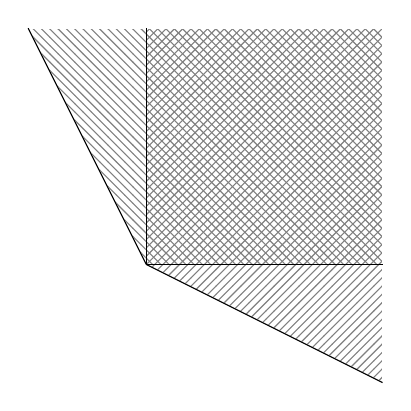
\begin{tikzpicture}
			\draw [color = white, pattern=north west lines, pattern color = gray] 
				(0,0) -- (-1.5,3) -- (3,3) -- (3,0) -- cycle; 
			\draw [color = white, pattern=north east lines, pattern color = gray]
				(0,0) -- (3,-1.5) -- (3,3) -- (0,3) -- cycle;
			\draw (0,0) -- (0,3);
			\draw (0,0) -- (3,0);
			\draw (0,0) -- (3,-1.5);
			\draw (0,0) -- (-1.5,3);
		\end{tikzpicture}
		\subcaption{An overlapping pair of monoids in $\Z^2$}
	\end{minipage}
	\hspace{30mm}
	\begin{minipage}{.3\textwidth}
		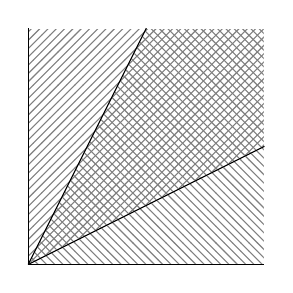
\begin{tikzpicture}
			\draw [color = white, pattern=north west lines, pattern color = gray] 
				(0,0) -- (1.5,3) -- (3,3) -- (3,0) -- cycle; 
			\draw [color = white, pattern=north east lines, pattern color = gray]
				(0,0) -- (3,1.5) -- (3,3) -- (0,3) -- cycle;
			\draw (0,0) -- (0,3);
			\draw (0,0) -- (3,0);
			\draw (0,0) -- (3,1.5);
			\draw (0,0) -- (1.5,3);
		\end{tikzpicture}
		\subcaption{The picture of associated dual cones of the overlapping pair.}
	\end{minipage}
\end{center}
\end{figure}
 Another property of morphisms that will be useful is that of being exact.
\begin{defn}
	A morphism $f:P\to Q$ of monoids is said to be exact provided the following diagram
	$$\xymatrix{
		P \ar[r]^{f}\ar[d] & Q\ar[d]\\
		P^{gp}\ar[r]^{f^{gp}} & Q^{gp}
		}$$
	is cartesian. 
\end{defn}
It is immediate from this definition that $f$ is exact precisely when $x\leq y$ if and ony if $f(x)\leq f(y)$ for any $x, y\in P$. 

A certain type of monoid, a \emph{valuative} monoid, plays a very similar role in the study of monoids and cones as that of a valuation ring in the study of commutative rings and schemes. 
\begin{defn}\label{valMon}
	A sharp monoid $M$ is said to be valuative if for any $x\in M^{gp}$, either $x$ or $-x$ is an element of $M$.
\end{defn}
Sharp morphisms from monoids to valuative monoids will be of particular interest. Given a morphism of monoids $f:P\to Q$, we get an associated morphism of cones $f^*:\Cone(P)\to \Cone(Q)$. Suppose that $Q$ is valuative, say $Q = \NN$, then the morphism on cones gives a ray in $\Cone(P)$. To say that $f$ is sharp is to say that this ray does not land in any face of the cone $\Cone(P)$. By (\cite{Ogus}, (1.1.7)) every monoid $P$ induces a partial order on its associated group $P^{gp}$ by acting by translation. We may equivalently define a sharp monoid to be valuative provided this partial order is actually a total order.
\begin{lem}
	Let $M$ be a sharp monoid. The following are equivalent
	\begin{align*}
		(i) & \; M\text{ is valuative}\\
		(ii) & \; \text{The partial order induced on }M^{gp}\text{ by }M\text{ is a total order}.
	\end{align*}
\end{lem}
\begin{proof}
	First assume that $M$ is valuative, and let $x,y\in M^{gp}$. Then $x-y\in M^{gp}$ and hence $x-y\in M$ or $-(x-y)\in M$ since $M$ is valuative. Since under this partial ordering $M$ is the monoid of positive elements in $M{gp}$, it is either the case that $x-y\geq 0$ or $y-x\geq 0$, that is either $x\geq y$ or $y\geq x$ and hence $M^{gp}$ is totally ordered. 
	
	Conversely assume that the partial order induced on $M^{gp}$ by $M$ is a total order and let $x\in M^{gp}$. Then in particular either $x\geq 0$ or $x\leq 0$ which is equivalent to saying that $x\in M$ or $-x\in M$. 
\end{proof}

 Notice that we did not include the adjective \emph{saturated} in the definition of a valuative monoid. This is because a valuative monoid is always saturated.
\begin{lem}
	Valuative monoids are saturated.
\end{lem}
\begin{proof}
	Let $M$ be a valuative monoid. Let $x\in M^{gp}$ such that $nx\in M$. Then, since we can view $M$ as the monoid of non-negative elements under the total order induced from the action of $M$ on $M^{gp}$, $nx\geq 0$. It follows immediately that $x\geq 0$ since $M^{gp}$ is totally ordered and hence $x\in M$, from which it follows that $M$ is saturated.
\end{proof}
The very definition of a smooth covering family relies on sharp morphisms to valuative monoids. Thankfully, these always exist.
\begin{lem}\label{sharpValMor}
	Any sharp, integral monoid $P$ admits a sharp morphism to a sharp valuative monoid with the same associated group.
\end{lem}
\begin{proof}
	Extend the partial order on $P^{gp}$ to a total order using (\cite{Marczewski}, pg. 387), and then take the maximal sharp monoid of elements $\geq 0$ inside of the group with the extended order. This will be a sharp valuative monoid admitting a sharp morphism from $P$.
\end{proof}
By (\cite{Ogus}, Lemma 2.2.2), in the event that $P$ is finitely generated, it suffices to take the valuative monoid whose existence is ensured by the lemma to be $\NN$. In fact, up to isomorphism, $\NN$ is the only finitely generated valuative monoid (\cite{Ogus}, Proposition 2.1.16). What is more, every sharp morphism to a sharp valuative monoid $P\to M$ factors through a sharp valuative monoid contained in $P^{gp}$ containing $P$.
\begin{lem}\label{valuativeFactorization}
	Let $f: P\to M$ be a sharp morphism to a sharp valuative monoid. Then $f$ factors through $P\subseteq M'$ for some sharp valuative monoid $M'$ contained in $P^{gp}$ containing $P$.
\end{lem}
\begin{proof}
	The group $M^{gp}$ is totally ordered by definition of a valuative monoid. Hence the morphism $f^{gp}:P^{gp}\to M^{gp}$ induces a total order on $P^{gp}$ by $x\leq y$ if and only if $f(x) \leq f(y)$. Let $M'$ be a maximal sharp monoid inside of $(f^{gp})^{-1}(M)$ containing $P$. Then $M'$ is a sharp valuative monoid contained in $P^{gp}$ containing $P$ such that the diagram
$$\xymatrix{
	& M' \ar[dr] & \\
	P \ar[ur]\ar[rr] & & M\\
	}$$
commutes, completing the proof.
\end{proof}

Let $P$, $Q$ be monoids and $M$ a valuative monoid, and let $P\to Q$ be a morphism of monoids. The morphism $P\to Q$ is said to be smooth at $Q\to M$ if for any commutative diagram 
\begin{center}
	$\xymatrix{
		P \ar[d]\ar[dr]\\
		Q\ar[r] & M
	}$
\end{center}
and any surjection of valuative monoids $M'\to M$ producing a commutative diagram of solid arrows
\begin{center}
	$\xymatrix{
		P\ar[r]\ar[d] & M'\ar[d]\\
		Q\ar[r] \ar@{-->}[ur] & M,
	}$
\end{center}
there exists a dashed arrow making the diagram commute. 

\begin{defn}
A family of morphisms $\{P\to Q_i\}_i$ is said to be a smooth covering family if for any valuative monoid $M$ and sharp morphism $P\to M$ there exists an $i$ such that $P\to Q_i$ is smooth at $Q_i\to M$.
\end{defn}

%Assuming that $P$ and $Q$ are finitegely generated in addition, we may reduce to the case that $M=M' = \NN$. Hence the right vertical arrow is simply multiplication by some integer. %If we ask for it to be surjective, then it must be the case that that integer is $1$ and hence we have reduced the diagram to having only $\NN$ in the top right corner, which is precisely %the case that we were in before... If we allow multiplication by $n$ on the right hand vertical arrow in the diagram, then we are in the case of universal surjectivity. We will indeed %demand that our families be universall surjective.

%We need an additional condition to define the notion of being an \'etale family. Let $M$ be a valuative monoid. We will say that a family $\{P\to Q_i\}_i$ is \'etale at $Q_i\to M$ if there exists $M'$ completing the diagram
%\begin{center}
%	$\xymatrix{
%		P \ar[r] \ar[d] & M' \ar[d]\\
%		Q_i \ar[r] \ar@{-->}[ur] & M\\
%	}$
%\end{center}

\begin{exm}
	There is a way to formalize ``infinitessimal motion" in the setting of monoids by using certain valuative monoids. This infinitessimal motion provides some intuition as to what geometric condition the smooth covering families should satisfy. To build this intuition, let us work with the dual cones of the monoids. Given a ray lying in the interior of the dual cone of a monoid, there should be some element of the cover that this ray factors through. Moreover, infinitessimal motion away from this ray in any direction should factor through this same element of the cover. For a concrete example, let $\NN[\epsilon]$ be the submonoid of $\Z + \Z[\epsilon]$ generated by $1$ and $1-n\epsilon$ for all $n\in\NN$. We observe that $\NN[\epsilon]^{gp} \cong \Z^2$. Given any $x\in\Z^2$ either $x$ or $-x$ will lie in $\NN[\epsilon]$, and thus $\NN[\epsilon]$ is a valuative monoid. 
\begin{figure}[h!]\label{FuzzyMonoid}
	\begin{center}
		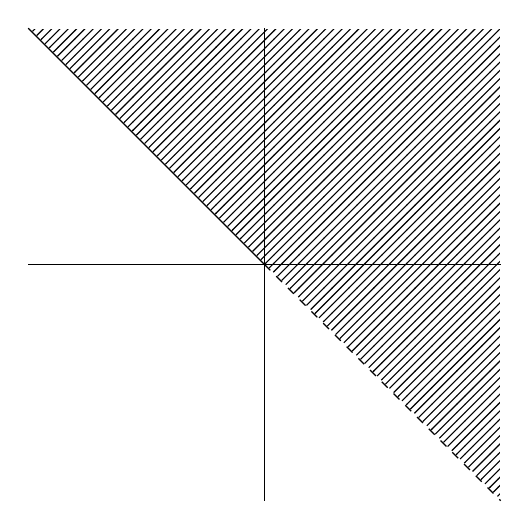
\begin{tikzpicture}
			\draw [color = white, pattern = north east lines]
				(0,0) -- (-3,3) -- (3,3) -- (3,-3) -- cycle;
		        \draw (0,-3) -- (0,3);
			\draw (-3,0) -- (3,0);
			\draw (0,0) -- (-3,3);
			\draw [dashed] (0,0) -- (3,-3);
		\end{tikzpicture}
		\caption{ The lattice points in the shaded region, along with the solid ray along the line passing through the origin and $(-1,1)$, comprise the monoid $\NN[\epsilon]$. We have mapped it into $\Z^2$ here by sending $\epsilon\mapsto (-1,1)$ and $1\mapsto (1,1)$.}
	\end{center}
\end{figure}	
	Let $f: \NN^2\to \NN[\epsilon]$ be any monoid morphism. Then, taking dual cones, we will get $f^*: \Cone(\NN[\epsilon])\to \Cone(\NN^2)$. We need only say what the generators pull back to under $f$ in order to specify the associated map on cones. Let $e_1 = (1,0)$ and $e_2 = (0,1)$ be a pair of generators for $\NN^2$. Define $f$ by $e_1\mapsto 1$ and $e_2\mapsto 1+\epsilon$. In order to describe $f^*$, we may describe where each of the dual functions $\epsilon^*$ and $(1-n\epsilon)^*$ gets sent in $\Cone(\NN^2)$. By definition of $f$, we have $e_2 - e_1\mapsto \epsilon\in\NN[\epsilon]$ and hence $\epsilon^*\mapsto e_1^* + e_2^*$. Similarly $e_1 - n(e_2 - e_1) = (n+1)e_1 - ne_2 \mapsto 1 - n\epsilon$ for all $n$, so that $(1-n\epsilon)^*\mapsto (n+1)e_1^* + n\epsilon^*$ for all $n$. We may envision this as a ray with a little bit of``infinitessimal motion" in the $e_2$ direction. The ray will pass through $(1,1)$ since $f^*(\epsilon^*) = e_1^* + e_2^*$.  
\begin{figure}[h!]\label{FuzzyCone}
	\begin{center}
		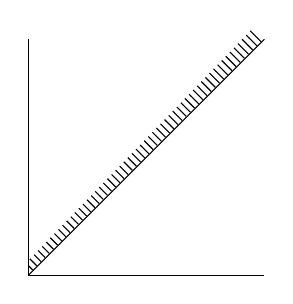
\begin{tikzpicture}
			\draw [color = white, pattern = north west lines]
				(0,0) -- (3,3) -- (2.84, 3.14) -- (0,0.2) -- cycle;
			\draw (0,0) -- (3,3);
			\draw (0,0) -- (0,3);
			\draw (0,0) -- (3,0);
		\end{tikzpicture}
		\caption{The "fuzz" extending from the ray passing through $(1,1)$ is coming from the $e_2$ direction.}
	\end{center}
\end{figure}
\end{exm}
\newpage

Smooth covering families are also exact covering families, as displayed in the following proposition.
\begin{prop}\label{smoothExactness}
	Let $\{P\xrightarrow{f_i} Q_i\}_{i\in I}$ be a smooth covering family. Then the morphism $f = (f_i)_{i\in I}:P\to\prod_{i\in I} Q_i$ is exact.
\end{prop}
\begin{proof}
Let $x,y\in P$ such that $f_i(x)\leq f_i(y)$ for all $y$. If $P$ is finitely generated then there exists a sharp morphism $g:P\to \NN$. Since the family lifts all sharp maps to $\NN$, there exists some $h = Q_i\to \NN$ so that $g = hf_i$. Hence $g(x)\leq g(y)$, which in turn implies that $g(y-x)\geq 0$, and therefore $x\leq y$ because $g$ is sharp. This will work if $P$ is not finitely generated as well, as if $P$ is any sharp, saturated, integral monoid then there exists a sharp morphism $P\to M$ for some valuative $M$. Therefore $P\to \prod_i Q_i$ is exact. 
\end{proof}
Smooth covering families also behave nicely with respect to pushouts along sharp morphisms.
\begin{lem}\label{smoothSharpPushouts}
	Let $\{P\to Q_i\}_{i\in I}$ be a smooth covering family. Let $P\to P'$ be a sharp morphism. Then $\{P'\to P'\oplus_P Q_i\}_{i\in I}$ is also a smooth covering family. 
\end{lem}
\begin{proof}
	Let $M$ be a valuative monoid and $P'\to M$ a sharp morphism. Then we get a sharp morphism $P\to M$ by composition. By definition of a smooth covering family, there thus exists a commutative diagram
$$\xymatrix{
	P\ar[dr]\ar[d] & \\
	Q_i\ar[r] & M }$$
for some $i$ such that for any valuative monoid $M'$ with a surjective morphism $M'\to M$ and any morphism $P\to M'$ there exists a commutative diagram of solid arrow
$$\xymatrix{
	P\ar[d]\ar[r] & M'\ar[d]\\
	Q_i\ar[r]\ar@{-->}[ur] & M }$$
such that the dotted arrow exists making the diagram commute. Now, applying the universal property of the pushout to the commutative diagram of solid arrows
$$\xymatrix{
	P\ar[r]\ar[d] & P' \ar@/^/[ddr]\ar[d] & \\
	Q_i\ar[r]\ar@/_/[drr]& Q_i\oplus_P P'\ar@{-->}[dr] &\\
	 & & M }$$
ensures the existence of the unique dotted arrow making the diagram commute. Again, applying the uniiversal property of the pushout to the commutative diagram of solid arrows
$$\xymatrix{
	P \ar[r]\ar[d] & P'\ar[r]\ar[d] & M'\\
	Q_i\ar[r]\ar[urr] & Q_i\oplus_P P'\ar@{-->}[ur]}$$
ensures the existence of a unique dotted arrow making the diagram commute. Putting these two diagrams together gives a commutative diagram of solid arrows
$$\xymatrix{
	P' \ar[r]\ar[d] & M'\ar[d]\\
	Q_i\oplus_P P'\ar[r]\ar@{-->}[ur] & M}$$
such that the dotted arrow exists making the diagram commute. This completes the proof.
\end{proof}



Let $A\to B$ be a smooth morphism of commutative rings. Then the induced morphism $\Omega_A\otimes_A B\to \Omega_B$ is a split injection. In the setting of commutative integral monoids, for a given monoid $P$, the groupification $P^{gp}$ of $P$ acts as the cotangent space of $P$. That is, we can think of $P^{gp}$ as ``$\Omega_P$". Applying this analogy, we arrive at a directly analogous statement for smooth morphisms of monoids.
\begin{lem}\label{splitInjection}
	Let $P\to Q$ be a morphism of monoids that is smooth at $Q\to M$ for some valuative monoid $M$. Then $P^{gp}\to Q^{gp}$ is a split injection.
\end{lem}
\begin{proof}
	We will first show that $P^{gp}\to Q^{gp}$ is injective. Let $g:P\to M$ be a sharp morphism to a valuative monoid and and $f:P\to Q$ is smooth at $h:Q\to M$. Let $g':P\to M^{gp} + \epsilon P^{gp}$ by $g'(x) = g(x) = \epsilon p$. Let $M$ be a valuative monoid in $M^{gp} + \epsilon P^{gp}$ containing the image of $P$. Then we obtain an induced surjective morphism $M'\to M$ from $\epsilon\mapsto 0$. Therefore the following diagram of solid arrows
\begin{equation}\label{splitLift}
\xymatrix{
	P\ar[r]\ar[d] & M'\ar[d]\\
	Q\ar^{h}[r]\ar@{-->}^{h'}[ur] & M\\
	}
\end{equation}
commutes, and the dotted arrow exists making the whole diagram commute. Now suppose $x\neq y$ in $P^{gp}$. Then $g'(x) = g'(y)$ since $\epsilon x\neq \epsilon y$. Now, as the diagram commutes we have that $h'(f(x)) = g'(x) \neq g'(y) = h'(f(y))$ from which it follows that $f(x)\neq f(y)$. 

	To see that $P^{gp}\to Q^{gp}$ is split, we make use of the diagram \eqref{splitLift} again. The morphism $h': Q^{gp}\to M^{gp} + \epsilon P^{gp}$ is defined by $h'(x) = h(x) + \epsilon s(x)$ where $s:Q^{gp}\to P^{gp}$ is a morphism satisfying $s(f(x)) = x$ for all $x\in P^{gp}$ by the commutativity of the diagram. That is to say that $s$ is a splitting of $f$, which completes the proof.
\end{proof}
As a direct corolloary to this Lemma, we may observe that smooth morphisms have torsion free quotients.
\begin{lem}\label{torsionFreeQuotient}
	Let $f:P\to Q$ be smooth at $Q\to M$. Then $Q^{gp}/P^{gp}$ is torsion free.
\end{lem}
\begin{proof}
	By Lemma \eqref{splitInjection}, the morphism $f:P^{gp}\to Q^{gp}$ admits a splitting $s:Q^{gp}\to P^{gp}$. Let $\overline{x}\in Q^{gp}/P^{gp}$ such that $n\overline{x} = 0$. Then $\overline{x}$ is represented by some $x\in Q^{gp}$ such that $nx = f(y)$ for some $y\in P^{gp}$. Therefore $ns(x) = y$ and hence $nfs(x) = nx$, from which we obtain
		$$n(fs(x) - nx) = 0.$$
Since $Q^{gp}$ is torsion free this implies that $fs(x) = x$ and hence  $x$ is in the image of $f$, that is to say $\overline{x} = 0$.
\end{proof}
Following Lemma \eqref{splitInjection}, we make the following definition.
\begin{defn}\label{injectiveFamily}
	We will say a family $\{P\to Q_i\}_{i\in I}$ is an injective family if $P\to Q_i$ is injective for all $i$.
\end{defn}
We will from this point on replace any smooth family with its injective torsion free covering subfamily -- that is, we will assume that each $f_i$ is injective and that each quotient $Q_i^{gp}/P^{gp}$ is torsion free. In particular, this implies that $P\to \prod_{i\in I}Q_i$ is injective. Therefore we only need to prove exactness of the sequence \eqref{sheafDescent} at $\prod_{i\in I}Q_i$. Example \eqref{notSat} shows that the associated group of the pushout of saturated monoids over a sharp morphism may have torsion. If that were the case, then there would be no hope of showing the exactness of \eqref{sheafDescent} in general. The lifting condition defining the smooth covering family forces torsion free cokernels.

A particularly useful observation is in order. Let $Q_i$ and $Q_j$ be any two monoids from a smooth covering family. Let $G = (Q_i\oplus_P Q_j)^{gp}$ and
	$$H = Q_i^{gp}\oplus_{P^{gp}} Q_j^{gp}\cong Q_i\oplus Q_j^{gp}/P^{gp}.$$
Then $G = H/H_{tor}$. As a corollary to the previous lemma, we may observe that $H_{tor} = \{0\}$.
\begin{cor}\label{noTorsion}
	With the notation as above, $H_{tor} = \{0\}$.
\end{cor}
\begin{proof}
	Let $x\in H$ such that $nx = 0$ for some $x$. Let $\overline{x}$ be the image of $x$ in the quotient group $H/Q_i^{gp}$. Then $x$ is still a torsion element, but by Lemma \eqref{torsionFreeQuotient} we have that $\overline{x} = 0$. And therefore $x\in Q_i^{gp}$. But $Q_i^{gp}$ is torsion free since $Q_i$ is saturated. Therefore $x = 0$, from which the result follows.
\end{proof}
Therefore we have the following isomoprhisms:
	$$(Q_i\oplus_P Q_j)^{gp} \cong Q_i^{gp}\oplus_{gp} Q_j^{gp} \cong Q_i^{gp}\oplus Q_j^{gp}/P^{gp}.$$
This property of smooth covering families will prove to be quite useful when proving the descent properties of the topology. An additional property that comes as a consequence of the definition of a smooth morphism of monoids is that lifts are forced to be sharp. \\
\begin{lem}\label{sharpLift}
	Let $P\to Q$ be smooth at $Q\to M$. Then $Q\to M$ is sharp.
\end{lem}	
\begin{proof}
	Let $g:P\to M$ be a sharp morphism such that the following diagram commutes
$$\xymatrix{
	P \ar[dr] \ar[d]& \\
	Q\ar[r] &M.\\}$$
Then let $h_1, h_2:P\to M^{gp} + eP^{gp}$ by $h_1(x) = g(x) + \epsilon x$ and $h_2(x) = g(x) - \epsilon p$ for $x\in P$. Let $M'$ be a valuative submonoid of $M^{gp} + \epsilon P^{gp}$ containing the image of $P$. Let $x\in Q$ such that $x\mapsto 0$ in $M$. Since $P\to Q$ is smooth at $Q\to M$ we have a commutative diagram of solid arrows
$$\xymatrix{
	P\ar[r]\ar[d] & M'\ar[d]\\
	Q\ar[r]\ar@{-->}[ur] & M,}$$
such that the dotted arrow exists making the diagram commute with either choice of $h_1$ or $h_2$ for the top arrow. Therefore we must have, choosing $h_1$, that $x\mapsto \epsilon p\in M'$ and choosing $h_2$ that $x\mapsto -\epsilon p\in M'$. Therefore $x=0$ from which it follows that $Q\to M$ is sharp. 
\end{proof}
Geometrically, from the perspective of cones, this is saying that any point in the interior of $P$ must factor through the interior of one of the elements in the cover -- it cannot factor through a face of every covering cone if it does not factor through a face of the cone being covered.

%Proof of descent for monoids.
\section{Descent Properties for Smooth Covering Families}
This section will be devoted to studying the following sequence:
\begin{center}
\begin{equation}\label{sheafDescent}
	$$\xymatrix{
		0\ar[r] & P\ar[r] \ar[d] & \prod_i Q_i\ar[r]\ar[d] & \prod_{i,j}Q_i\oplus_P Q_j \ar[d]\\
		0\ar[r] & P^{gp}\ar[r] & \prod_iQ_i^{gp}\ar[r] & \prod_{i,j}(Q_i\oplus_P Q_i)^{gp}.\\
	}$$
\end{equation}
\end{center}
In the next section, wherein we will show that taking smooth covering families to be covering forms a site on the category of sharply monoidal spaces, that the first row of this sequence is exact will imply that the topology is subcanonical. Indeed, this will show that each functor $\Cone(P)$ represented by $P$ is in fact a sheaf. Theorem \eqref{monoidDescent} contains the formal statement that utimately is the main player in this section.

%Two element covering family
\begin{lem}\label{twoElementCover}
	Suppose that $\{P\to Q_i\}_{i=1}^2$ is a smooth covering family. Then \eqref{sheafDescent} is exact.
\end{lem}
\begin{proof}
Suppose there is a monoid $P'$ equalizing the first row of \eqref{sheafDescent}. Then it must also equalize the second row. If we can show that the second row is exact, then we will obtain a factorization $P'\to P^{gp}$. By using the universal property of exactness of $P\to \prod_i Q_i$, we will then obtain a unique arrow $P'\to P$ making the whole diagram commute. We will then have shown that $P$ is the equalizer of the top row. On the level of groups, $(P^{sat})^{gp} = P^{gp}$ and $(P^{\sharp})^{gp} = P^{gp}/P^*$. Therefore 
	$$(Q_i\oplus_P Q_j)^{gp} \cong (Q_i\oplus_P Q_j)^{gp}/((Q_i\oplus_P Q_j)^{sat})^*.$$

The group $(P^{sat})^*$ is torsion by Lemma \eqref{torsionUnits}. Therefore if $(Q_1\oplus_P Q_2)^* = 0$ then $((Q_1\oplus_P Q_2)^{sat})^*$ is torsion. However, the assumption $P^{gp}\cong Q_1^{gp}\cong Q_2^{gp}$ implies that $Q_1\oplus _P Q_2$ is the sum $Q_1 + Q_2$ inside of $P^{gp}$, and $(Q_1 + Q_2)^{gp} \cong P^{gp} + P^{gp} = P^{gp}$. Thus it follows that $(Q_1\oplus_P Q_2)^{sat}$ is torsion free because $P^{gp}$ is torsion free by the assumption that $P$ is saturated. We therefore have that
\begin{equation}\label{sameGroupQuotient}
	(Q_1\oplus_P Q_2)^{gp} \cong P^{gp}/(Q_1 + Q_2)^*,
\end{equation}	
so in this case it suffices to show that $(Q_1 + Q_2)^* = 0$.

Let $z\in (Q_1 + Q_2)^*$. Then $z = q_1 +q_2$, subject to the condition that there exists some $q_1' + q_2'\in Q_1 + Q_2$ such that $(q_1 + q_2) + (q_1' + q_2') = 0$. Rearranging, we see that $q_1 + q_1'\in Q_1 $ has an inverse $q_2 + q_2'\in Q_2$. By symmetry, $q_2+q_2'$ has an inverse in $Q_1$. Therefore in the event that $(Q_i + Q_j)^*\neq 0$, neither morphism $\pi_i,\pi_j:Q_i,Q_j \to Q_i\oplus_P Q_j$ will be sharp. We note that $(Q_i +Q_i)^* = 0$, so we need only consider $i\neq j$. 

By Lemma \eqref{sharpValMor} there exists a valuative monoid $M$ and a sharp morphism $Q_1 + Q_2\to M$. By the universal property of the pushout, we get a diagram
\begin{center}
	$\xymatrix{
		P \ar[r]^{f_2}\ar[d]^{f_1}\ar[dr]^{h} & Q_2\ar[d]^{g_2}\\	
		Q_1\ar[r]^{g_1} & M.\\
	}$
\end{center}
The map from the pushout to $M$ is sharp, so $h^{gp}(y) = g_1^{gp}(y) = g_2^{gp}(y) = 0$, where here we are viewing $y$ as an element of each of the three isomorphic groups $P^{gp}$, $Q_1^{gp}$, and $Q_2^{gp}$ simutaneously. Define $M[\epsilon]^{gp} = M^{gp}\times \epsilon P^{gp}$. We obtain a morphism $f: P^{gp}\to M[\epsilon]^{gp}$ by $f(p) = h^{gp}(p) + \epsilon p$ for any $p\in P^{gp}$. Let $M'$ be any valuative monoid in $M[\epsilon]^{gp}$ containing the image of $P$. Then we have a morphism $P\to M'$, to which we will also refer as $f$. Thus this produces a commutative diagram of solid arrows
\begin{center}
	$\xymatrix{
		P\ar[r]^{f}\ar[d]^{f_i} & M'\ar[d]\\
		Q_i \ar[r]^{g_i} \ar@{-->}[ur]^{h_i'} & M,\\
	}$
\end{center}
for $i = 1,2$, such that the dotted arrow exists, and where the morphism $M'\to M$ is induced from $M[\epsilon]^{gp}\to M^{gp}$ by $\epsilon\to 0$. Now since the diagram is commutative we have that 
	$$h_1'(f_1(y)) = h(y) + \epsilon y\qquad\text{and}\qquad h_2'(f_2(-y)) = -(h(y) + \epsilon y).$$
But $M'$ is sharp so that $h(y) + \epsilon y = 0$, from which it follows that $y = 0$ since $f$ is a sharp morphism. It follows that $(Q_1 + Q_2)^* = 0$ and hence \eqref{sheafDescent} is exact. 
\end{proof}
As discussed, we now remove the hypothesis that there are only two elements in the cover, while retaining for the time being the assumption that the ambient groups are the same. First, we require a lemma.
\begin{lem}\label{sameGrpPush}
	Assume that $P$, $Q$, and $Q'$ are objects in $(\Mon^{sat})^{\sharp}$, $P\to Q$ and $P\to Q'$ are sharp, and $P^{gp}\cong Q^{gp} \cong Q'^{gp}$. Then the following are equivalent:
	\begin{align*}
		1) & \;Q \text{ and } Q' \text{ are an overlapping pair,}\\
		2) & \;(Q + Q')^* = 0.\\
	\end{align*}	
\end{lem}
\begin{proof}
	If $P^{gp}\cong Q^{gp} \cong Q'^{gp}$ then $Q\oplus_P Q'= Q + Q'$, taken in $P^{gp}$. There is a nonzero element $q_1 + q_1'\in (Q+Q')^*$ if and only if there is some $q_2 + q_2'\in Q + Q'$ such that $q_1 + q_1' + q_2 + q_2' = 0$ and hence $q_1 + q_2$ is an element of $Q$ that has an inverse in $Q'$. This is precisely the statement that the map $Q\to Q\oplus_P Q'$ is not sharp, and hence that that $Q$ and $Q'$ are not an overlapping pair.  
\end{proof}
Geometrically, this is saying that the intersection of the cones has a non-empty relative interior precisely when they do not intersect in a face.

%arbitrary cover, same groups
\begin{lem}\label{ArbCovSameGrp}
	Let $\{P\to Q_i\}_{i\in I}$ be a smooth covering family with $P^{gp}\cong Q_i^{gp}$ for all $i$. Then \eqref{sheafDescent} is exact.
\end{lem}
\begin{proof}
Applying the isomorphisms $Q_i^{gp}\cong Q_j^{gp} \cong P^{gp}$ for each $i$ and $j$ and equation \eqref{sameGroupQuotient} gives us the isomorphisms
	$$(Q_i\oplus_P Q_j)^{gp} \cong P^{gp}/(Q_i + Q_j)^*$$
for all $i$ and $j$. Now, the morphism $\prod_i P^{gp} \rightarrow \prod_{i,j}P^{gp}/(Q_i + Q_j)^*$, coming from the above isomorphisms and the bottom row of the sequence \eqref{sheafDescent},
takes the $i^{th}$ and $j^{th}$ component of $x$ to $x_i - x_j$. Suppose that the image of $x$ under this morphism is $0$, that is $x_i - x_j \in (Q_i + Q_j)*$ for all $i$ and $j$. We make use of the following.


Consider the relation $\sim$ on the index set $I$ of the covering family defined by $i\sim j$ if and only if $(Q_i + Q_j)^* = 0$  (\emph{Note: the relation is symmetric and reflexive but not transitive; it is not necessarily an equivalence relation on $I$}). To see that \eqref{sheafDescent} is exact, it will suffice to show that $\sim$ is connected. We may build a graph $\Gamma$ out of this relation on the index set as follows. Include a vertex $v_i$ for every element $Q_i$ of the covering family. Then include an edge between $v_i$ and $v_j$ whenever $i\sim j$. To show that $\sim$ is connected amounts to showing that $\Gamma$ is connected. 

Let $x\in P^{gp}$ such that $x,-x\not\in P$. Choose some monoid $Q$ from the covering family. If for every $x\in Q$, there does not exist any $Q'$ in the covering family for which $-x\in Q'$, then $Q$ forms an overlapping pair with all $Q'$. If this is the case, then $\Gamma$ is connected, from which we conclude that \eqref{sheafDescent} is exact. Otherwise, there exists some $Q'$ and some $x\in Q$ such that $-x\in Q'$. Now define the subgraphs $\Gamma^+$ and $\Gamma^-$ of $\Gamma$ as follows:
	$$\Gamma^+ = \{v_i\mid -x\not\in Q_i\},\qquad \Gamma^- = \{v_i\mid x\not\in Q_i\}.$$
To say that such $Q$, $x$, and $Q'$ exist is to say that there is some $v\in \Gamma^+\setminus \Gamma^-$ and $v'\in \Gamma^-\setminus\Gamma^+$. We have proven exactness of \eqref{sheafDescent} in the event that the cover consists of two monoids. Now assume that the graph $\Gamma$ is connected in the event that the cover consists of up to $N$ monoids. Then suppose that there are $N+1$ monoids in the covering family. Since each of $P\to P[x]$ and $P\to P[-x]$ are sharp morphisms, both of the families
	$$\{P[x]\xrightarrow{f_{i,x}} Q_i[x]\}_{v_i\in\Gamma^+} \qquad\text{and}\qquad \{P[-x]\xrightarrow{f_{i,-x}} Q_i[-x]\}_{ v_i\in\Gamma^-}$$
are smooth covering by lemma \eqref{smoothSharpPushouts}. Moreover, since each of $\Gamma^+$ and $\Gamma^-$ are strictly smaller than $\Gamma$, it follows that each of the families is strictly smaller than the original family. Thus we may apply induction to deduce that each of $\Gamma^+$ and $\Gamma^-$ are connected. 

	There exists a sharp valuative monoid $M$, and a sharp morphism $f_x: P[x,-x]\to M$. Since $x,-x\not\in P$ by design, the morphism $f: P\to M$ is also sharp. Therefore there exists some $Q_i$ such that $P\to Q_i$ has the lifting property at $Q_i\to M$. Let $M[\epsilon]^{gp} = M^{gp}\times \epsilon P^{gp}$, and consider the morphism $P\to M[\epsilon]^{gp}$ defined by $p\mapsto (f(p), \epsilon p)$. Then choose any valuative monoid $M'\subseteq M[\epsilon]^{gp}$ containing the image of $P[x]$. This naturally induces a commutative diagram
$$\xymatrix{
	P[x] \ar[r]\ar[d] & M'\ar[d]\\
	Q_i[x] \ar[r]\ar@{-->}[ur] & M,\\
	}$$
where under the dotted arrow, we will have $x\mapsto \epsilon x$. Therefore it must not be the case that $-x\in Q_i$ since otherwise $-x\mapsto -\epsilon x$ under the dotted arrow, but $M'$ is sharp which forces the image of $x$ to actually be zero. It follows then that $-x\not\in Q_i$. Likewise, if we repeat this argument with $M'$ containing the image of $P[-x]$, then we may conclude that $x\not\in Q_i$. It follows that $v_i\in \Gamma^+\cap \Gamma^-$ and hence $\Gamma$ is connected, from which it follows that the sequence \eqref{sheafDescent} is exact. 
\end{proof}


%arbitray cover, different groups
\begin{thm}\label{monoidDescent}
	Let $\{P\to Q_i\}_{i\in I}$ be a smooth covering family. Then the sequence
		$$0\to  P\to \prod_i Q_i\rightrightarrows \prod_{i,j}Q_i\oplus_P Q_j$$
is exact. 
\end{thm}
\begin{proof}
For each $i$, let $Q_i' = (f_i^{gp})^{-1}(Q_i)$. Then each $P\to Q_i'$ is an exact morphism with $(Q_i')^{gp} \cong P^{gp}$ for all $i$, and $P\to Q_i$ factors through $P\to Q_i'$ for all $i$, from which it follows immediately that $\{P\to Q_i'\}_i$ is an smooth covering family. Therefore by Lemma \eqref{ArbCovSameGrp}, the sequence
	$$0\to P\to \prod_i Q_i'\rightrightarrows \prod_{i,j} Q_i'\oplus_P Q_j'$$
is exact. Furthermore, this gives us a morphism of sequences
\begin{equation}\label{monSeqMap}
	\xymatrix{
		0 \ar[r] & P\ar[r]\ar[d] & \prod Q_i' \ar@<-.25pc>[r]\ar@<.25pc>[r]\ar[d] & \prod_{i,j} Q_i'\oplus_P Q_j'\ar[d]\\
		0 \ar[r] & P \ar[r] & \prod_i Q_i\ar@<.25pc>[r] \ar@<-.25pc>[r] & \prod_{i,j} Q_i\oplus_P Q_j.\\
	}
\end{equation}
We have isomorphisms $Q_i'^{gp}\cong P^{gp}$ for all $i$, and $(Q_i'\oplus_P Q_j')^{gp} \cong P^{gp}/(Q_i' + Q_j')^*$ for all $i,j$. Following from Lemma \eqref{splitInjection}, each $P\to Q_i$ is injective, and hence it is also the case that $\prod_i Q_i'^{gp}\to \prod_i Q_i^{gp}$ is injective. Now, applying the isomorphism $(Q_i' \oplus_P Q_j')^{gp} \cong P^{gp}/(Q_i' + Q_j')^*$ we get morphisms
	$$P^{gp}/(Q_i' + Q_j')^* \to (Q_i\oplus_P Q_j)^{gp}$$
for all $i$ and $j$. Applying the groupification functor to \eqref{monSeqMap}, we obtain the following diagram
\begin{equation}\label{groupSequence}
	\xymatrix{
		 & 0\ar[d] & 0\ar[d] & \\
		0 \ar[r] & P^{gp}\ar[r]\ar@{=}[d] & \prod Q_i'^{gp} \ar[r]\ar^{h}[d] & \prod_{i,j} P^{gp}/(Q_i'+Q_j')^*\ar^{h'}[d]\\
		0 \ar[r] & P^{gp} \ar[r]\ar[d] & \prod_i Q_i^{gp}\ar@<.25pc>[r] \ar@<-.25pc>[r]\ar[d] & \prod_{i,j} (Q_i\oplus_P Q_j)^{gp}\\
		& 0 & \prod_i (Q_i\oplus_{Q_i'} Q_i)^{gp} & .\\
	}
\end{equation}
By the proof of Lemma \eqref{ArbCovSameGrp}, wherein we showed the connectivity of $\sim$, for each $i$ there exists some $j$ such that $(Q_i' + Q_j')^* = 0$ and hence we obtain morphisms $P^{gp}\to (Q_i \oplus_P Q_j)^{gp}$ for all such $i$ and $j$. This will be useful in proving the following, the proof of which we postpone until after the proof of the theorem..
\begin{lem}\label{injMorphism}
	The morphism $h'$ is injective.
\end{lem}	

Let $x = (x_i)_i\in\prod_i Q_i$ such that $x_i - x_j = 0$ in each $(Q_i\oplus_P Q_j)^{gp}$. From Corollary \eqref{noTorsion}, we have
	$$(Q_i\oplus_P Q_i)^{gp} \cong Q_i^{gp}\oplus_{P^{gp}} Q_i^{gp}\cong Q_i^{gp}\oplus Q_i^{gp}/P^{gp}$$
for all $i$. Therefore, by the middle column of \eqref{groupSequence}, for each $i$ there is an exact sequence
	$$0 \to Q_i'^{gp}\to Q_i^{gp}\to Q_i^{gp}\oplus Q_i^{gp}/Q_i'^{gp}.$$
Hence $x_i\mapsto 0\in Q_i^{gp}/P^{gp}$ for each $i$, from which it follows that $x_i\in Q_i'^{gp} \cong P^{gp}$ for all $i$. Then, since $h'$ is injective by Lemma \eqref{injMorphism}, the preimage $h'^{-1}(x_i-x_j)$ is also zero. As the top row is exact, we deduce that $(f_i^{gp})^{-1}(x_i) = x\in P^{gp}$ for all $i$. Finally, the morphism $P\to Q_i$ factors through $Q_i'$ for all $i$, from which we conclude that the bottom row of \eqref{groupSequence} is exact. 

	Consider now the diagram
$$
	\xymatrix{
		0 \ar[r] & P \ar[r]\ar[d] & \prod_i Q_i\ar@<.25pc>[r]\ar[d] \ar@<-.25pc>[r] & \prod_{i,j} Q_i\oplus_P Q_j \ar[d]\\
		0 \ar[r] & P^{gp} \ar[r] & \prod_i Q_i^{gp}\ar@<.25pc>[r] \ar@<-.25pc>[r] & \prod_{i,j} (Q_i\oplus_P Q_j)^{gp}.\\
	}
$$
Take any monoid $M$ that equalizes the top row. Then it will also equalize the bottom row producing a commutative diagram
$$
	\xymatrix{
		M \ar@/^/[drr] \ar@/_/[rdd] \ar@{-->}[dr]  & & \\
		& P \ar[r] \ar[d] & \prod_i Q_i\ar[d]\\
		& P^{gp} \ar[r] & \prod_i Q_i^{gp}\\
	}
$$
of solid arrows. Since smooth covering families are exact, the square is cartesian and hence by the universal property of the fibered product we get a unique dotted arrow showing that $P$ is the equalizer of the top row, which completes the proof of the theorem.
\end{proof}
We now provide the proof that was omitted from the statement of the Lemma during the proof of Theorem \eqref{monoidDescent}.
\begin{proof}[Proof of Lemma \eqref{injMorphism}]
	Let $i$ and $j$ be a indices such that $(Q_i' + Q_j')^* = 0$. Then we have a commutative diagram of solid arrows
$$\xymatrix{
	P^{gp} \ar^{\rotatebox{0}{$\sim$}}[r]\ar^{\rotatebox{90}{$\sim$}}[d] & Q_i'^{gp}\ar^{\rotatebox{270}{$\sim$}}[d]\ar[r] & Q_i^{gp}\ar[dd]\\
	Q_i'^{gp} \ar^{\rotatebox{0}{$\sim$}}[r]\ar[d] & (Q_i' + Q_j')^{gp}\ar@{-->}[dr] & \\
	Q_j^{gp}\ar[rr] & & (Q_i\oplus_P Q_j)^{gp}
	}$$
with a unique dotted arrow coming from the universal property of the pushout. By \cite{StacksProj}, Lemma 12.5.13 since the morphism $P^{gp}\to Q_j^{gp}$ is injective, then so is $Q_i^{gp}\to (Q_i\oplus_P Q_j)^{gp}$. Moreover, the diagonal morphism in the top left square of the diagram is an isomorphism $P^{gp}\to P^{gp}$. Hence, since the diagram commutes, the dotted arrow is the composition of $P^{gp}\cong P^{gp} \to Q_i^{gp} \to (Q_i\oplus_P Q_j)^{gp}$, which is therefore injective. For every $i$ there exists a $j$ such that $(Q_i' + Q_j')^* = 0$, from which it follows that $h'$ is injective.
\end{proof}

\section{Formally \'Etale for Sharp and Saturated Monoids}
	In analogy with the definitions of formally smooth and formally \'etale morphisms of schemes, if we ask for the lifts appearing in the definition of a formally smooth morphism of monoids to be unique, we arrive at the definition of a formally \'etale morphism. Let $P$ and $Q$ be monoids, given with morphisms $P\to Q$, and $P\to M$ for a valuative monoid $M$. We will say that $P\to Q$ is formally \'etale at $Q\to M$ if the diagram
$$\xymatrix{
	P\ar[d]\ar[dr] & \\
	Q\ar[r] & M\\
	}$$
commutes and for any valuative monoid $M'$ with a surjective morphism $M'\to M$ and any sharp morphism $P\to M'$ the following diagram of solid arrows
$$\xymatrix{
	P\ar[d]\ar[r] & M'\ar[d]\\
	Q\ar[r]\ar@{-->}[ur] & M}$$
commutes, and there exists a unique dotted arrow making the diagram commute. Just as we did for formally smooth morphisms, we can extend this notion to a formally \'etale covering family of monoids.
\begin{defn}
	A family of monoid morphisms $\{P\to Q_i\}_{i\in I}$ is said to be formally \'etale if for any sharp morphism $P\to M$ to a valuative monoid, there exists some $i$ such that $P\to Q_i$ is formally \'etale at $Q_i\to M$.
\end{defn}
Again, we may think of the associated group $P^{gp}$ of a monoid $P$ as the cotangent space to $\Cone(P)$. Recall from algebraic geometry that if a moprhism of rings $A\to B$ is \'etale then it is the case that $\Omega_A\cong \Omega_B$. We have the analogous statement in the case of monoids.
\begin{lem}
	Let $P\to Q$ be formally \'etale at $Q\to M$. Then $P^{gp}\cong Q^{gp}$.
\end{lem}
\begin{proof}
	Let $M'$ be a valuative monoid with a surjective morphism $M'\to M$, and let $P\to M'$ be any sharp morphism such that the diagram of solid arrows
$$\xymatrix{
	P\ar[r]\ar[d] & M'\ar[d]\\
	Q\ar[r]\ar@{-->}[ur] & M}$$
commutes. Denote by $\calL(Q,M')$ the collection of dotted arrows, i.e. lifts, that make the whole diagram commute. Suppose there is some lift $h\in \calL(Q,M')$. Given any lift $h'\in \calL(Q,M')$ we may produce an element $\varphi_{h'}\in\Hom(Q^{gp}/P^{gp}, M'^{gp})$ by $\varphi_{h'} = h'-h$. This morphism has a two sided inverse given by $\varphi_{h'} \mapsto \varphi_{h'} + h$. Therefore $\calL(Q, M') \cong \Hom(Q^{gp}/P^{gp}, M'^{gp})$ provided that $\calL(Q, M')\neq\empty$. However by assumption that $P\to Q$ is formally \'etale at $Q\to M$ we have that $\calL(Q, M') = 0$ and hence $\Hom(Q^{gp}/P^{gp}, M'^{gp}) = 0$ which implies that $Q^{gp}/P^{gp}$ is a torsion group since $M'^{gp}$ is torsion free ($M'$ is valuative). By Lemma \eqref{torsionFreeQuotient} $Q^{gp}/P^{gp}$ is torsion free and hence $Q^{gp}/P^{gp} = 0$.
\end{proof}

\begin{lem}
	Let $f:P\to Q$ be formally smooth at $Q\to M$ for some valuative monoid $M$. Then there exists a sharp valuative monoid $Q'$ such that $P\to Q'$ is formally \'etale at $Q'\to M$ and such that $Q'\to Q$ has a section. 
\end{lem}
\begin{proof}
	By \eqref{splitInjection} there exists a section $s:Q^{gp}\to P^{gp}$. Let $Q' = s(Q)$. It is clear that $Q'\to Q$ has a section, and thus we need only show that $P\to Q'$ is formally \'etale at $Q'\to M'$. We first note that $(Q')^{gp}\cong P^{gp}$. Let $M'\to M$ be surjective with $M'$ valuative and such that we have a commutative diagram of solid arrows
$$ \xymatrix{
	P\ar[r]\ar[d] & M'\ar[dd]\\
	Q' \ar@{-->}[ur]\ar[d] & \\
	Q \ar[r]\ar@{-->}[uur] & M.
	}$$
The dotted arrow $Q'\to M$ exists and makes the diagram commute by hypothesis, and hence there exists an arrow $Q'\to M'$ making the diagram commute by composition. However, the set $\calL$ of lifts $Q'\to M$ is in bijection with the set $\Hom((Q')^{gp}/P^{gp}, M'^{gp}) = 0$ and hence $\calL = 0$ from which it follows that the morphism $P\to Q'$ is formally \'etale. 

\end{proof}

\todo{finite presentation hypothesis}

%Topology for Sharply Monoidal Spaces
\section{The Smooth Topology For Sharply Monoidal Spaces}
	A sharply monoidal space is something like a shadow of a log scheme. Informally, if we forget about the scheme structure we simply retain a topological space with a sheaf of monoids, which is exactly what a monoidal space is. A sharply monoidal space is characterized additionally by the properties of morphisms in the category -- we require the induced morphisms on sheaves to be sharp at all stalks. This is very reminiscent of the situation from algebraic geometry wherein we have ringed spaces and locally ringed spaces. Formally, a sharply monoidal space is a pair $(X, \calM_X)$ consisting of a topological space and a sheaf of monoids $\calM_X$ and such that given any other locally monoidal space $(Y, \calM_Y)$ and a moprhism $f:X\to Y$ the induced morphism on stalks
		$$\calM_{Y, f(x)}\to \calM_{X,x}$$
is sharp for any $x\in X$.
\begin{exm}
	Let $P$ be an object in $(\Mon^{sat})^{\sharp}$. Then the pair $(\Cone(P), P)$ is an example of a locally monoidal space, with the topology given by taking covers to be smooth covering families. 
\end{exm}
Translating the definition of a smooth covering family of monoids to sharply monoidal spaces, we arrive immediately at the definition of a smooth covering family of locally monoidal spaces. First we tranlate the definition of being smooth at a point.
\begin{defn}
	Let $f: X\to Y$ be a morphism of sharply monoidal spaces. Let $M$ be a valuative monoid and let $\Cone(M)\to X$.....\todo{finish this}....
\end{defn}	

		
\begin{thebibliography}{9}

\bibitem[ACP]{TropCurve} Dan Abromovich, Lucia Caporaso, Sam Payne, \emph{The Tropicilization of the Moduli Space of Curves}, Ann. Sci. \'Ec Nom. Super. (4) 48 (015), no. 4, 765-809

\bibitem[AO]{Ogus} Arthur Ogus, \emph{Lectures on Logarithmic Algebraic Geometry}, September 15, 2006

\bibitem[CCUW]{CCUW} Renzo Cavalieri, Melody Chan, Martin Ulirsch, Jonathan Wise,\emph{ A Moduli Stack of Tropical Curves}, arXiv:1704.03806v1, April 12, 2017

\bibitem[K]{Kato} F. Kato, \emph{Log Smooth Deformation and Moduli of Log Smooth Curves}, International Journal of Mathematics, November 1999

\bibitem[LU]{LinUl} Bo Lin, Martin Ulirsch, \emph{Towards a Tropical Hodge Bundle}, arXiv:1701.04385, January 16, 2017

\bibitem[EM]{Marczewski} Edward Marczewski (1930), \emph{Sur l'extension de l'ordre partiel} (PDF), Fundamenta Mathematicae, 16: 386?389

\bibitem[CMV]{ChanSiegel} Melodie Chan, Margarida Melo, Filipo Viviani, \emph{Tropical Teichmuller and Siegel Spaces}, arXiv:1207.2443, July 10, 2012

\bibitem[MW]{MolchoWise} Samouil Molcho, Jonathan Wise, \emph{The Logarithmic Picard Group and its Tropicalization}, arXiv:1807.11364, July 30, 2018

\bibitem[Sta]{StacksProj} The Stacks Project Authors, \emph{stacks project}, http://stacks.math.columbia.edu, 2017

\bibitem[TT]{LogSchemes} Takeshi Tsuji, \emph{Saturated Morphisms of Logarithmic Schemes}, Research Institure for Mathematical Sciences, Kyoto Univesity, June 30, 1997

\bibitem[WG]{LogGeo} W.D Gillam, \emph{Log Geometry}, Department of Mathematics, Brown University, January 13, 2009

\bibitem[Fans]{Fans} W.D. Gillam, \emph{Fans}, arXiv:1601.02421, January 16, 2011

\end{thebibliography}

\end{document}
